\newproblem{14a}
{
	Graph the given equation. Be sure to label axis with x, y, and with numbers. Identify and label the x-intercept, y-intercept, and another point on the line.
	$$4y+8x=16$$
	\begin{onlyproblem}\begin{center}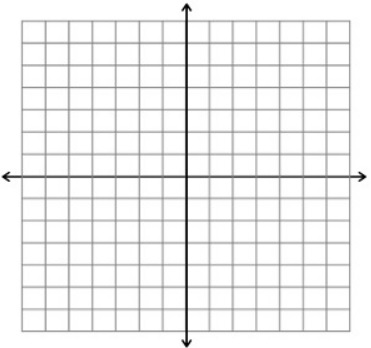
\includegraphics{fig-graphpaper.png}\end{center}\end{onlyproblem}
	\begin{onlysolution}\begin{center}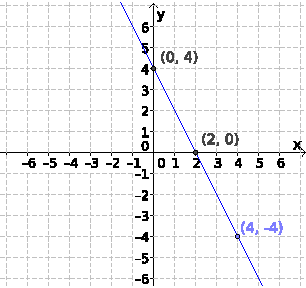
\includegraphics{fig095-09-a-answer}\end{center}\end{onlysolution}
}
{
	\begin{tabular}{l r}
	$(2,0)$ x-int & 2 pts\\
	$(0,4)$ y-int & 2 pts\\
	$(1,2),(-1,6),(3,-2),(-2,8)$ et al. & 2 pts\\
	x and y axis labeled & 1 pt\\
	graph & 1 pt\\
	\end{tabular}
}

\newproblem{14b}
{
	Graph the given equation. Be sure to label axis with x, y, and with numbers. Identify and label the x-intercept, y-intercept, and another point on the line.
	$$5y+2x=-10$$
	\begin{onlyproblem}\begin{center}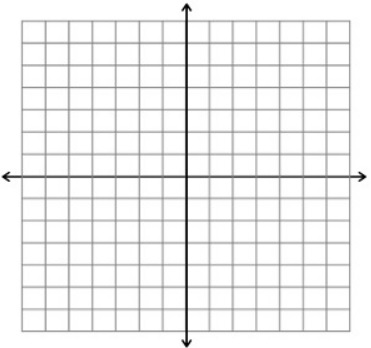
\includegraphics{fig-graphpaper.png}\end{center}\end{onlyproblem}
	\begin{onlysolution}\begin{center}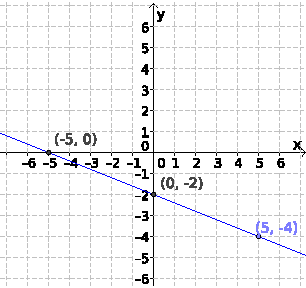
\includegraphics{fig095-09-b-answer}\end{center}\end{onlysolution}
}
{
	\begin{tabular}{l r}
	$(-5,0)$ x-int & 2 pts\\
	$(0,-2)$ y-int & 2 pts\\
	$(5,-4)$ et al. & 2 pts\\
	x and y axis labeled & 1 pt\\
	graph & 1 pt\\
	\end{tabular}
}

\newproblem{14c}
{
	Graph the given equation. Be sure to label axis with x, y, and with numbers. Identify and label the x-intercept, y-intercept, and another point on the line.
	$$-4y+3x=-12$$
	\begin{onlyproblem}\begin{center}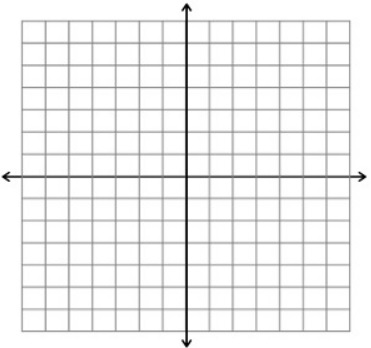
\includegraphics{fig-graphpaper.png}\end{center}\end{onlyproblem}
	\begin{onlysolution}\begin{center}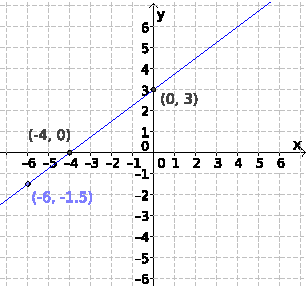
\includegraphics{fig095-09-c-answer}\end{center}\end{onlysolution}
}
{
	\begin{tabular}{l r}
	$(-4,0)$ x-int & 2 pts\\
	$(0,3)$ y-int & 2 pts\\
	$(4,6)$ et al. & 2 pts\\
	x and y axis labeled & 1 pt\\
	graph & 1 pt\\
	\end{tabular}
}

\newproblem{14d}
{
	Graph the given equation. Be sure to label axis with x, y, and with numbers. Identify and label the x-intercept, y-intercept, and another point on the line.
	$$4y-2x=12$$
	\begin{onlyproblem}\begin{center}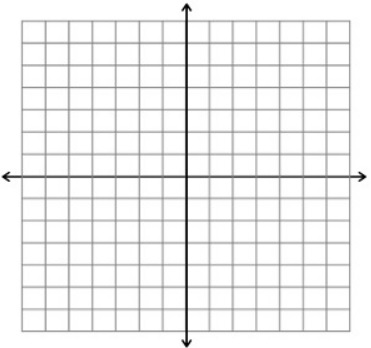
\includegraphics{fig-graphpaper.png}\end{center}\end{onlyproblem}
	\begin{onlysolution}\begin{center}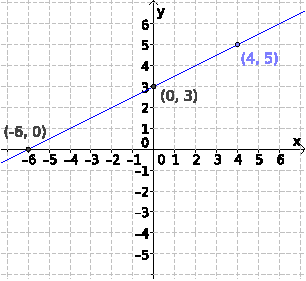
\includegraphics{fig095-09-d-answer}\end{center}\end{onlysolution}
}
{
	\begin{tabular}{l r}
	$(-6,0)$ x-int & 2 pts\\
	$(0,3)$ y-int & 2 pts\\
	$(-4,1),(-2,2),(2,4),(4,5),(6,6)$ et al. & 2 pts\\
	x and y axis labeled & 1 pt\\
	graph & 1 pt\\
	\end{tabular}
}
